%!TEX program = xelatex
\documentclass[12pt,oneside]{book}  % Remove draft option to show figures (for final draft), otherwise keep for faster production
\usepackage[UTF8]{ctex}
\usepackage{indentfirst}
\usepackage{uorthesis}  % Loads the LaTeX style package
\usepackage[backend=biber, style=authoryear]{biblatex}
\addbibresource{references.bib}
\usepackage{uorbib}
\usepackage{listings}
\usepackage{color,xcolor}
\usepackage{fontspec}
\usepackage{xeCJK}
\setmonofont[Mapping={}]{Menlo}    %英文引号之类的正常显示,相当于设置英文字体
\setsansfont{Menlo} %设置英文字体 Menlo, Consolas,  Fantasque Sans Mono
\setmainfont{Menlo} %设置英文字体
\setCJKmainfont{PingFang SC}
% Put custom packages to be loaded here
% \usepackage{linguex}  % For linguistic examples
% \usepackage{tikz}     % For drawing

\begin{document}

% Title page
\begin{titlepage}
  \vspace*{\fill}

  \begin{center}
    {\Huge Report of SLAM project \par
    }

    \bigskip%
    by

    \bigskip%
    Mingke Wang

    %%%%%

    \bigskip\bigskip\bigskip\bigskip%
    % Submitted in Partial Fulfillment of the

    \bigskip%
    % Requirements for the Degree

    \bigskip%
    Bachelor

    %%%%%

    \bigskip\bigskip\bigskip\bigskip%
    % Supervised by your supervisor

    \bigskip\bigskip%
    School of Electronic Information\\
    and Electrical Engineering\\

    %%%%%

    \bigskip\bigskip\bigskip\bigskip%
    Shanghai Jiao Tong University

    \bigskip%
    Shanghai, China

    %%%%%

    \bigskip\bigskip\bigskip\bigskip%
    2020
  \end{center}

  \vspace*{\fill}
\end{titlepage}

% All subsequent pages must be numbered, title page is considered page i,
% front matter is numbered in lowercase Roman numerals
\pagestyle{fancy}
\pagenumbering{roman}
\setcounter{page}{2}
\doublespacing

% Dedication (optional)
% \thispagestyle{plain}

\begin{center}
  \vspace*{\fill}

  \it%
  To whomever

  \vspace*{\fill}
\end{center}

\clearpage

% Acknowledgments
% \chapter*{\centerline{Acknowledgments}}
\markboth{\MakeUppercase{Acknowledgments}}{}
\iftoggle{fulltoc}{
  \addcontentsline{toc}{chapter}{Acknowledgments}
}{}

This thesis is the final project of class EE378, and the main topic I choose is quantum cryptography.

% Abstract
% \chapter*{\centerline{Abstract}}
\markboth{\MakeUppercase{Abstract}}{}
\iftoggle{fulltoc}{
  \addcontentsline{toc}{chapter}{Abstract}
}{}

In this artical, I mainly talk about what is quantum, how does it related to transmission cryptography, and the drawback of it.


% Table of Contents, List of Tables, List of Figures
\tableofcontents

%List of Tables & Figures
% % LIST OF TABLES & FIGURES

% List of tables, if applicable
\listoftables
\iftoggle{fulltoc}{
  \addcontentsline{toc}{chapter}{List of Tables}
}{}

% List of figures, if applicable
\listoffigures
\iftoggle{fulltoc}{
  \addcontentsline{toc}{chapter}{List of Figures}
}{}


%%%%%%%%%%%%%%%%%%%% DISSERTATION CONTENT %%%%%%%%%%%%%%%%%%%%

% Regular numbering starts now, first page of first chapter is page 1
\clearpage
\setcounter{page}{0}
\pagenumbering{arabic}

% Body


\chapter{Introduction}
\label{chap:introduction}

\section{Problem Introduction}
通过本课程的学习,我们知道通过若干张图像,我们可以同时获得图像中所拍摄场景的三维信息,并得到图像拍摄时的6个自由度的姿态和位置。

本课程大作业问题内容是使用自己的手机或相机,对同一个场景,分别在三个角度拍摄三张图像,最终获得三张图像拍摄时的姿态和位置,以及图像中特征点的三维坐标信息,并评估和验证所实现算法的正确性和精度性能。在本次实验中,我使用iphone手机拍摄的照片为交大“庙门”。三张图片如图所示:

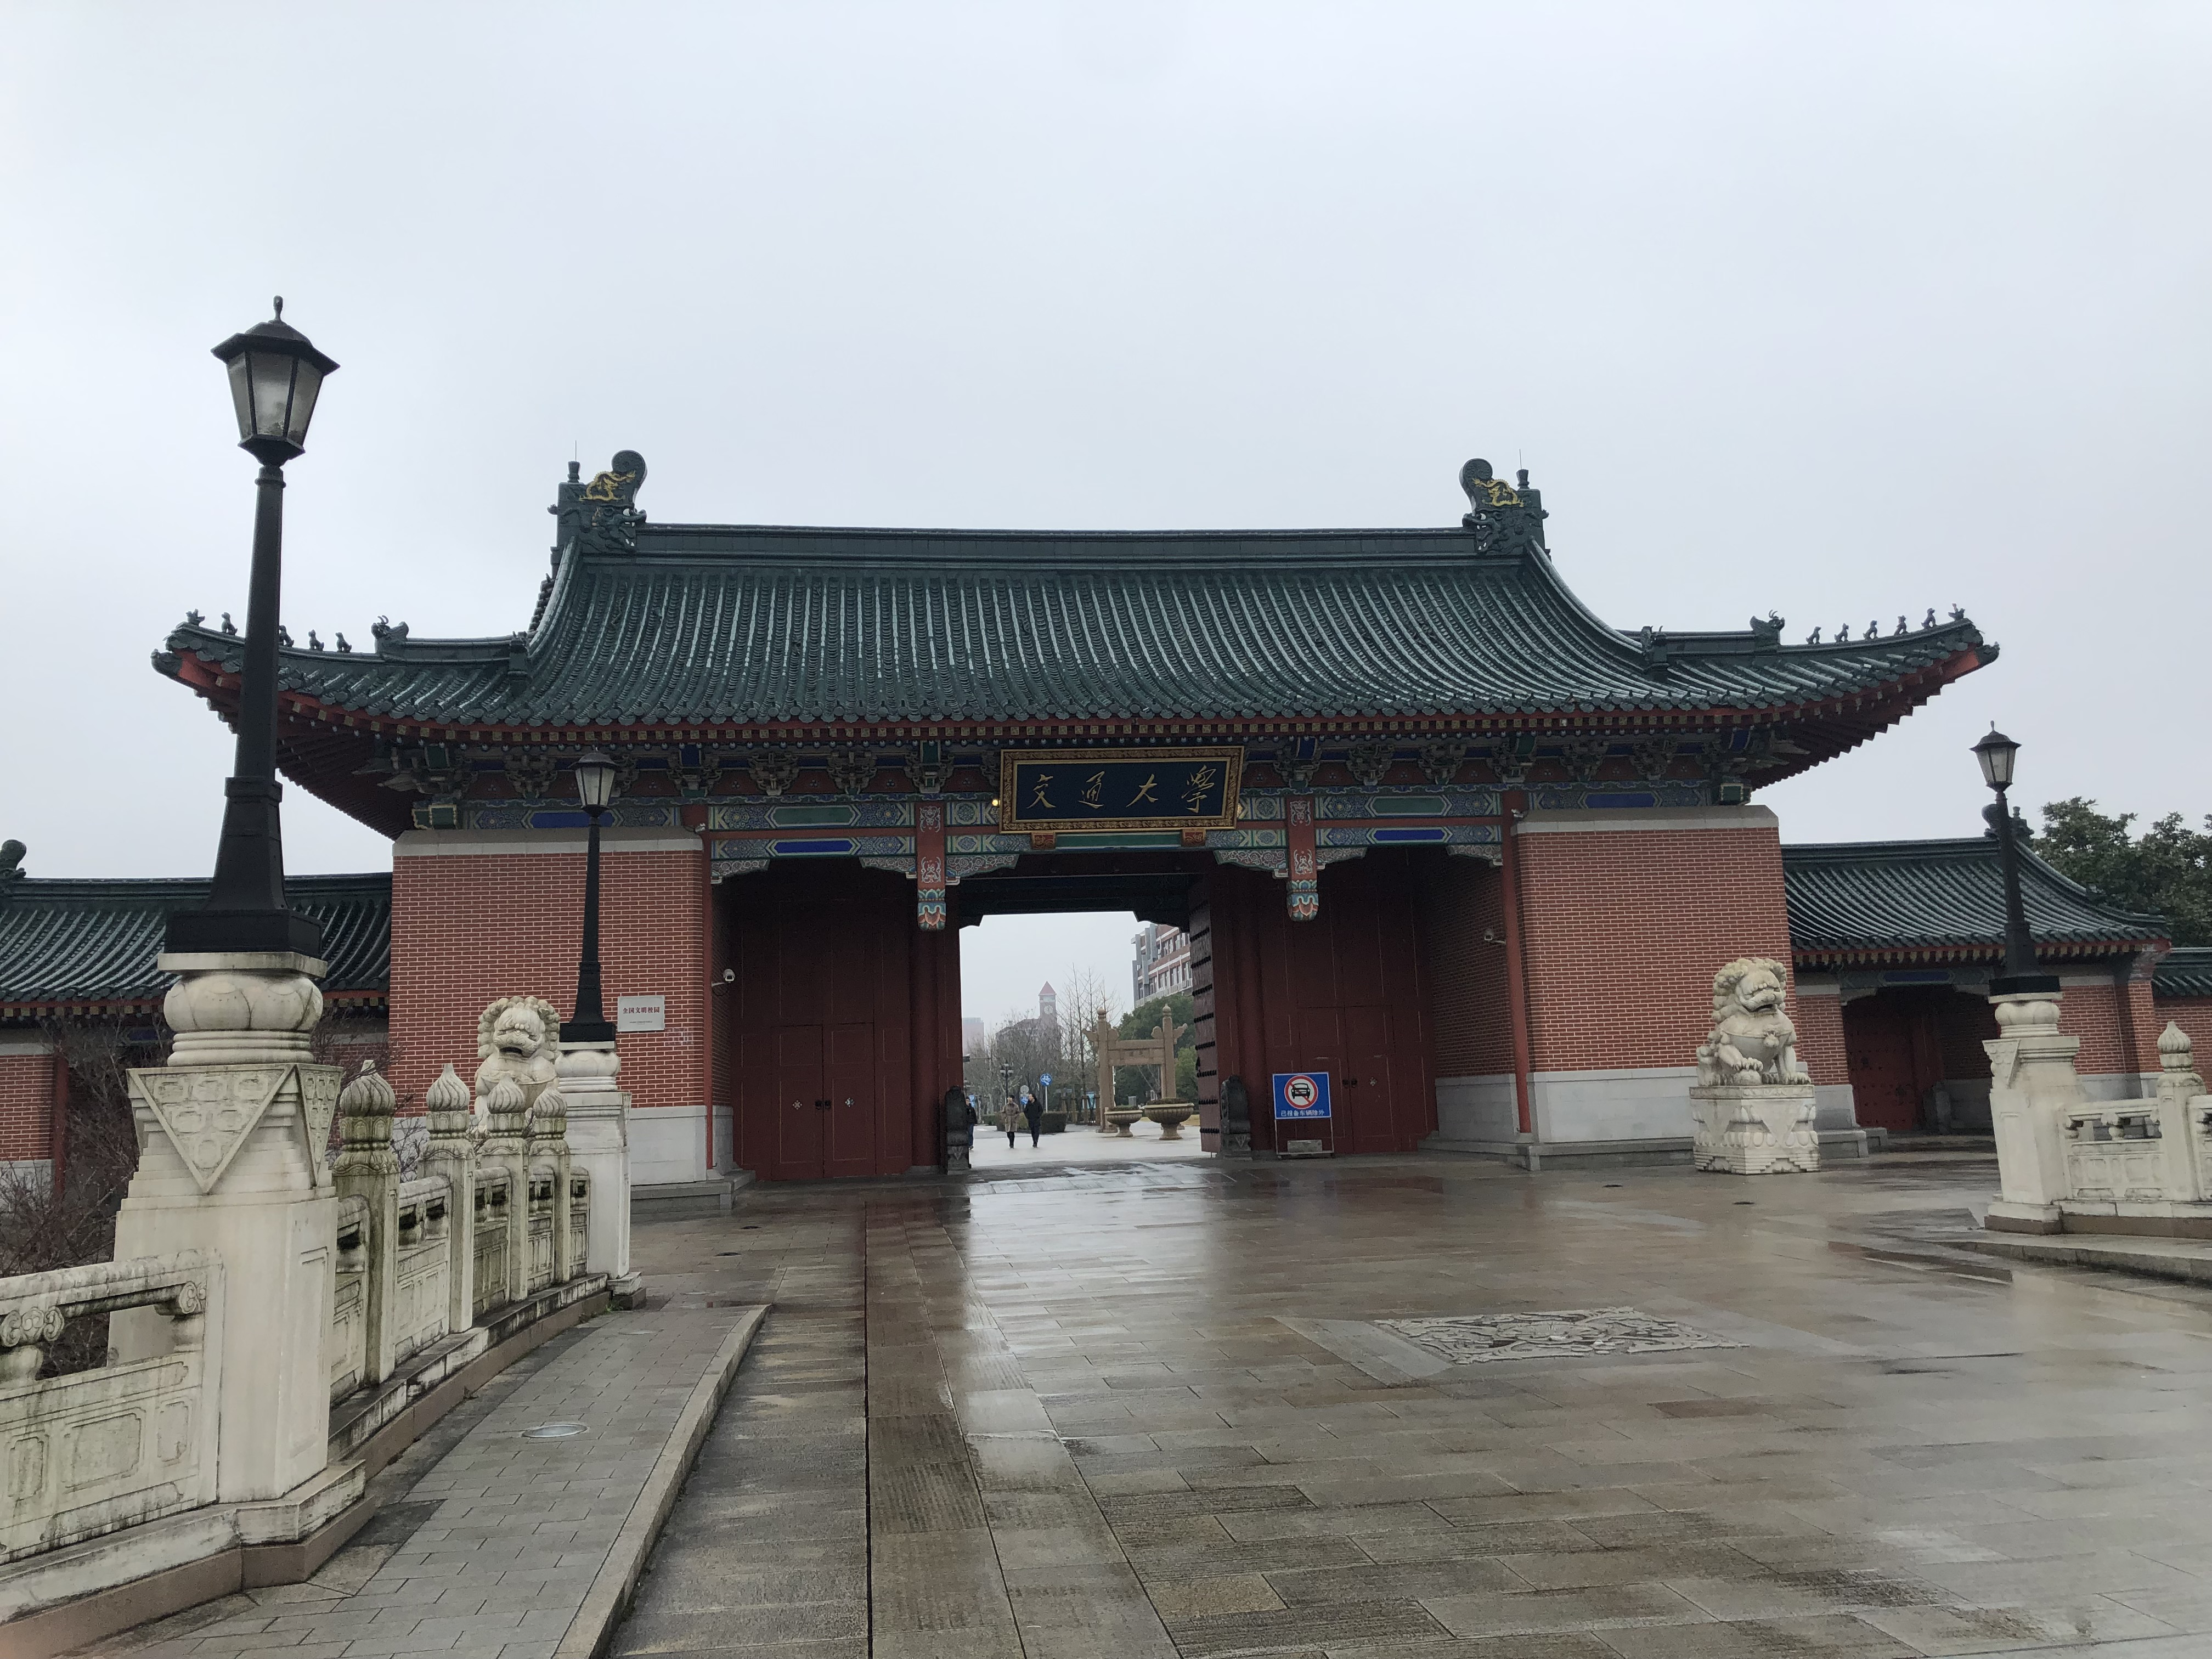
\includegraphics[width=0.3\textwidth]{/mnt/ff3bee5c-da50-4d90-848f-2a69bb4db3c8/HomeWork/SLAM_Project/1.JPG}
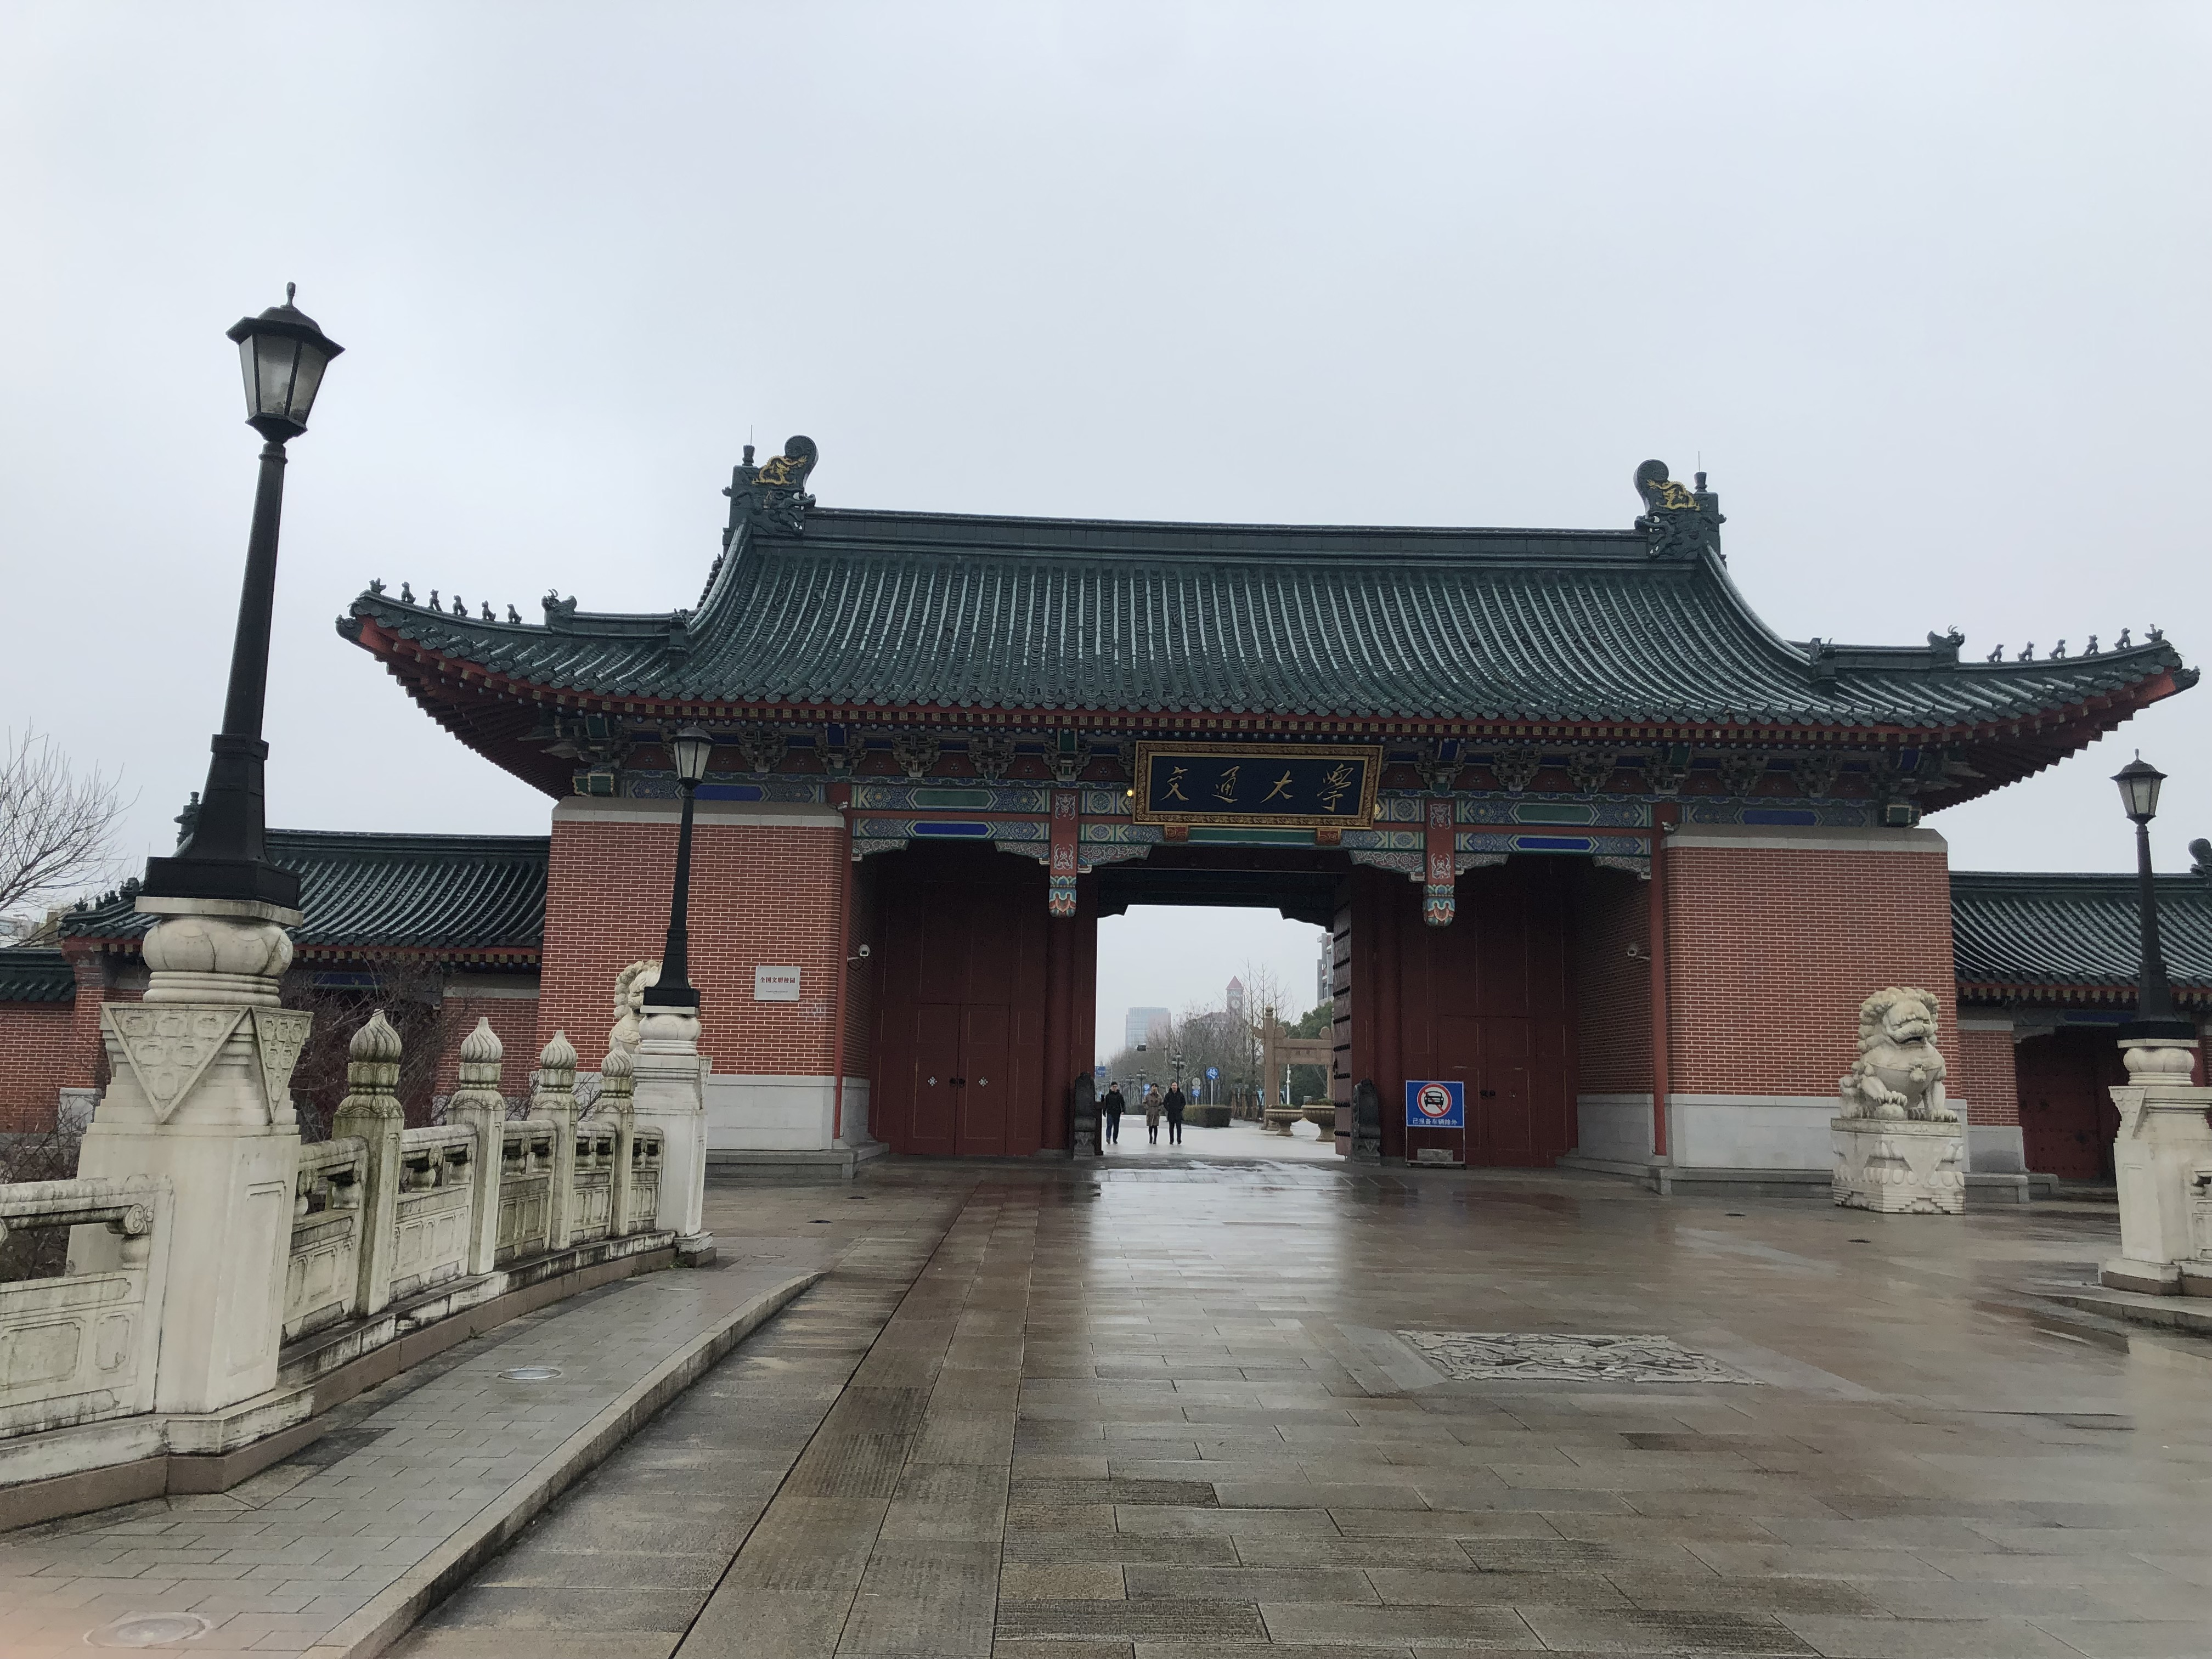
\includegraphics[width=0.3\textwidth]{/mnt/ff3bee5c-da50-4d90-848f-2a69bb4db3c8/HomeWork/SLAM_Project/2.JPG}
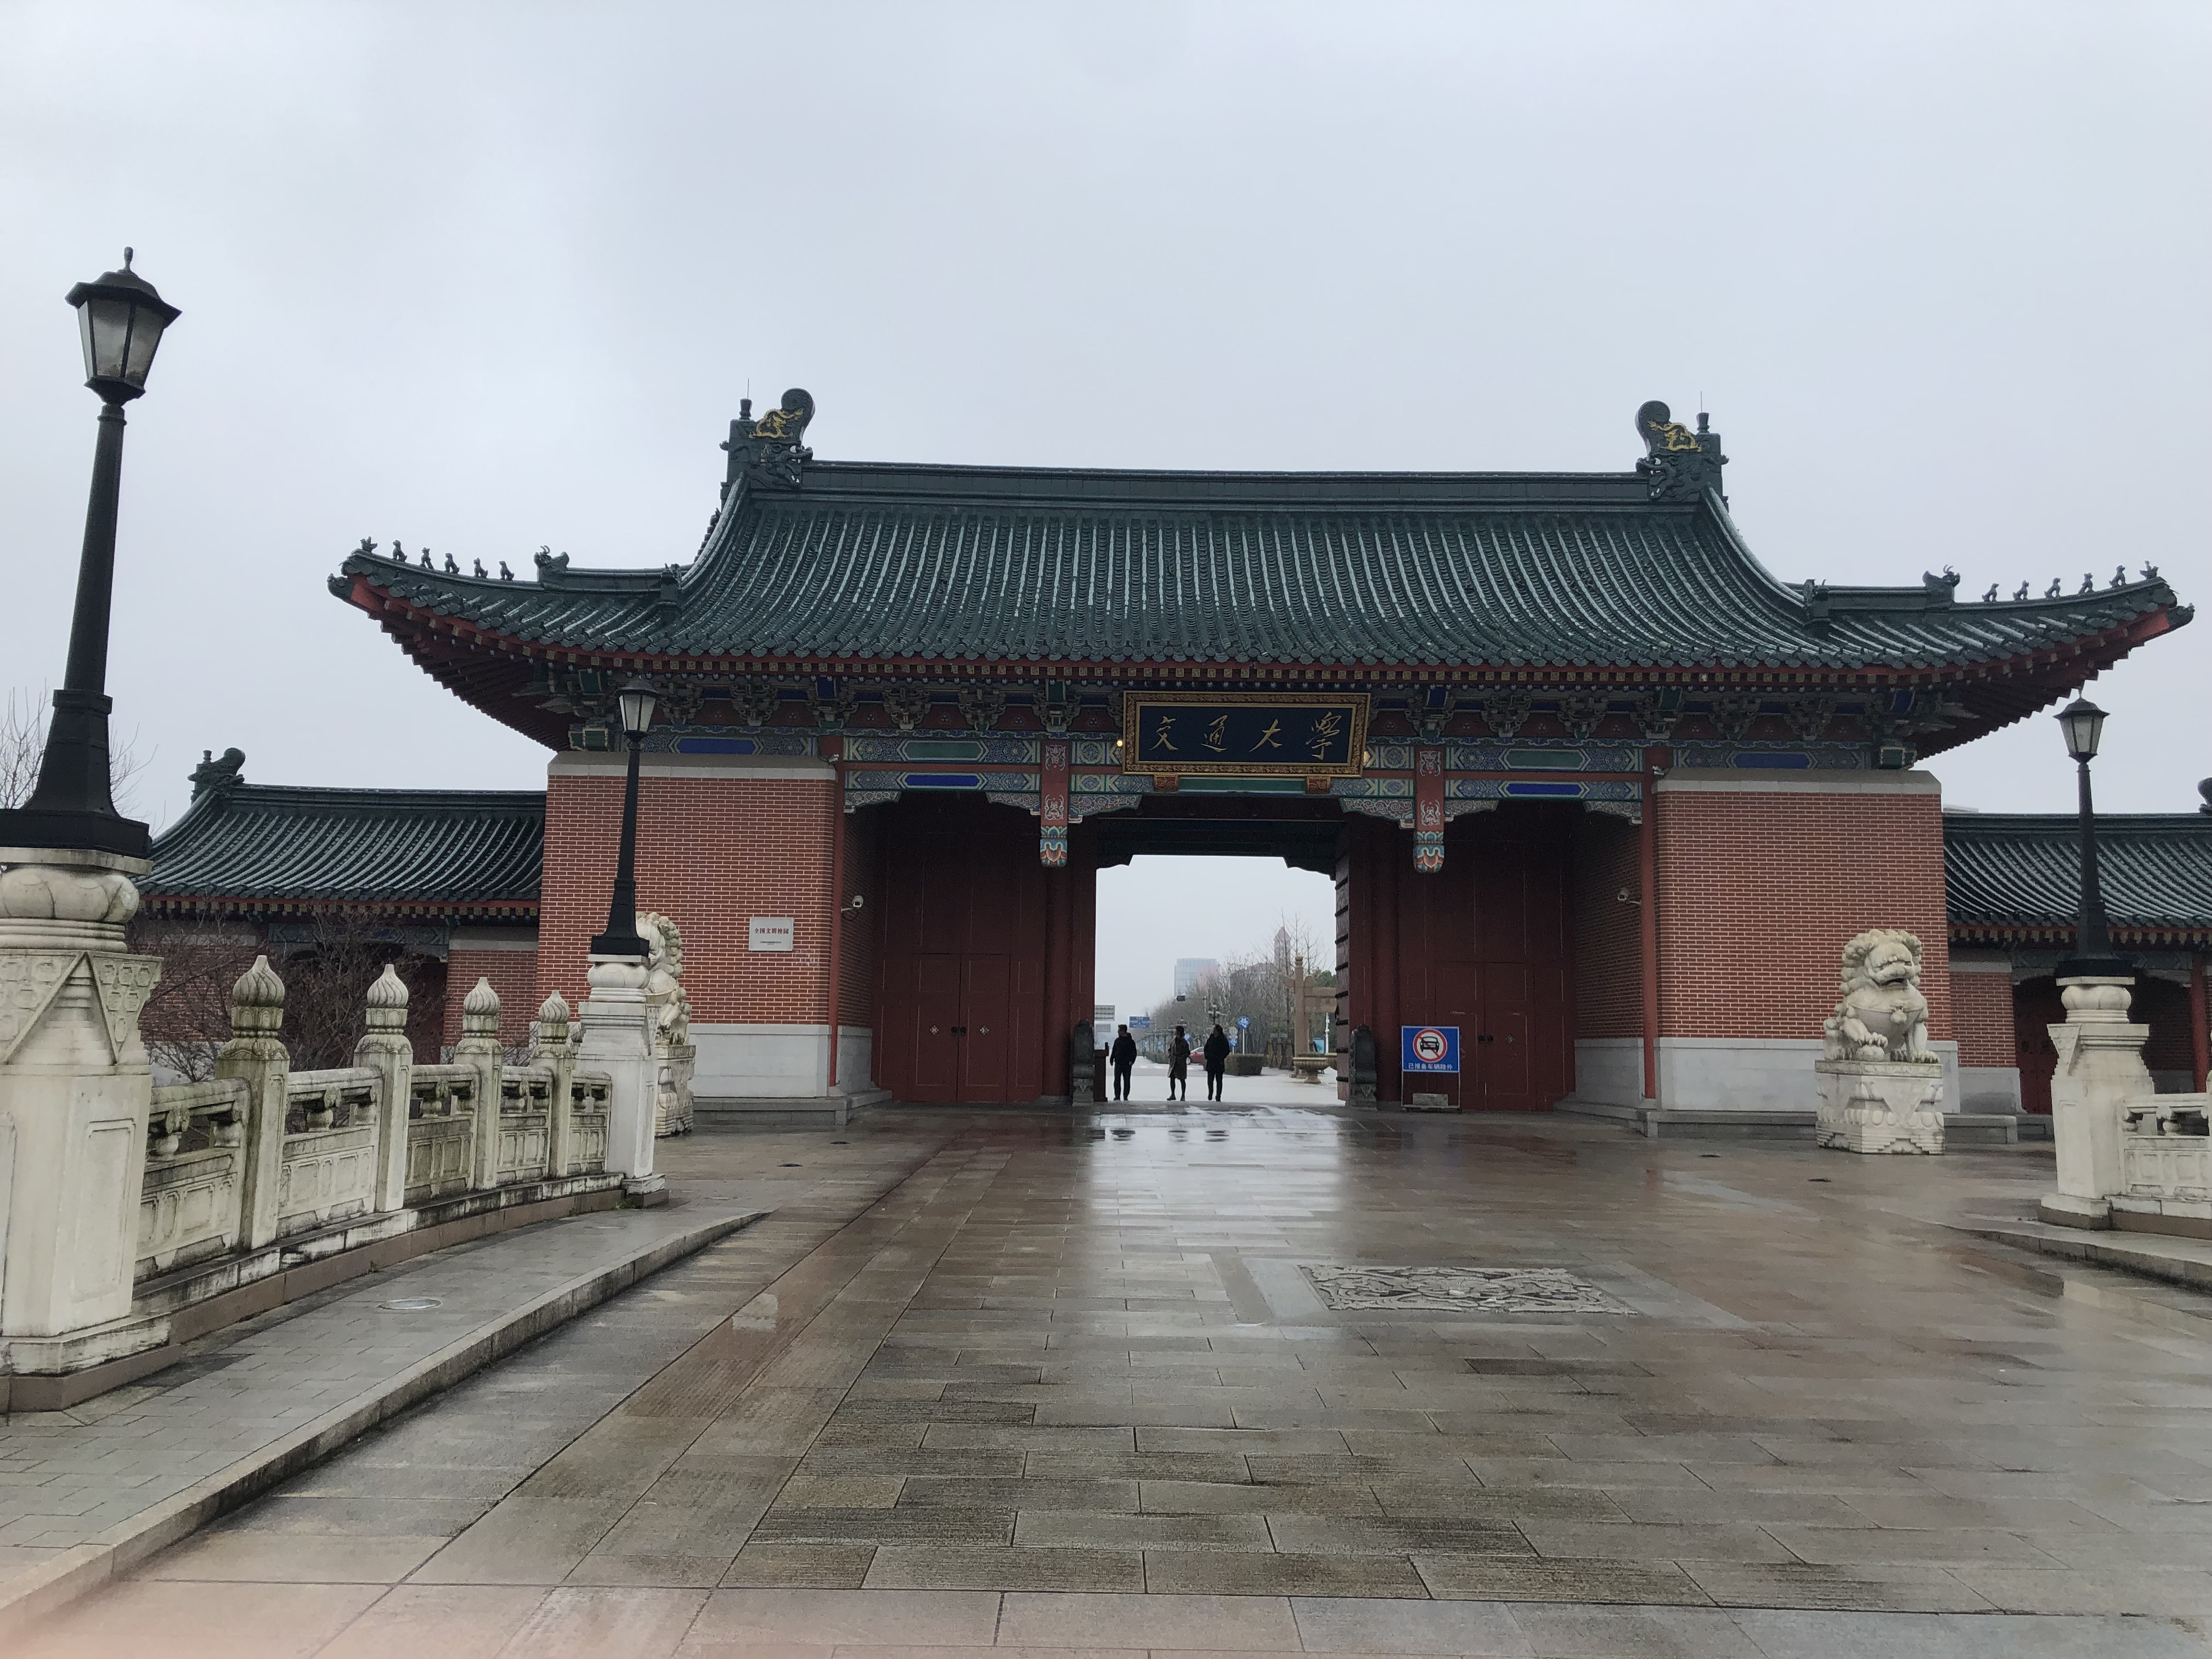
\includegraphics[width=0.3\textwidth]{/mnt/ff3bee5c-da50-4d90-848f-2a69bb4db3c8/HomeWork/SLAM_Project/3.JPG}

注:在拍摄时,所选择的场景纹理丰富,并且三维结构突出;三个拍摄角度间既要有足够的基线,也要控制相互夹角不大于30度,不然会造成后续特征点匹配的困难。

实验过程为利用拍摄的三张图片估计三次拍照的相对位姿。在实验过程中以第一次拍照的位置为轴,用相对旋转矩阵与平移矩阵来表示另外两次拍照的位姿。



\chapter{Theory}
\label{chap: Theory}

\section{Theory Overview}
首先选择其中两张照片,通过特征点匹配基础矩阵或本征矩阵的求解得到两个拍摄视角的相对位姿,然后使用三角化得到对应特征点的三维点云。对于第三张图,我们可通过相机位姿估算的方式求解其姿态和位置。在这里用的方法是通过第一张图片与第三张图片的特征点与三角化的三维点云的3D-2D匹配关系,利用RANSAC方法实现第三个视角的相机位置姿态估算。

\section{Theory Detail}
\subsection{相机内参标定}
通过MATLAB工具箱进行相机内参标定,需要用同一个相机对某个图案(这里选择黑白棋盘)拍摄多个位姿的图片,按照官方示例进行标定。其中拍摄的20张黑白棋盘的位姿图片如图4所示:

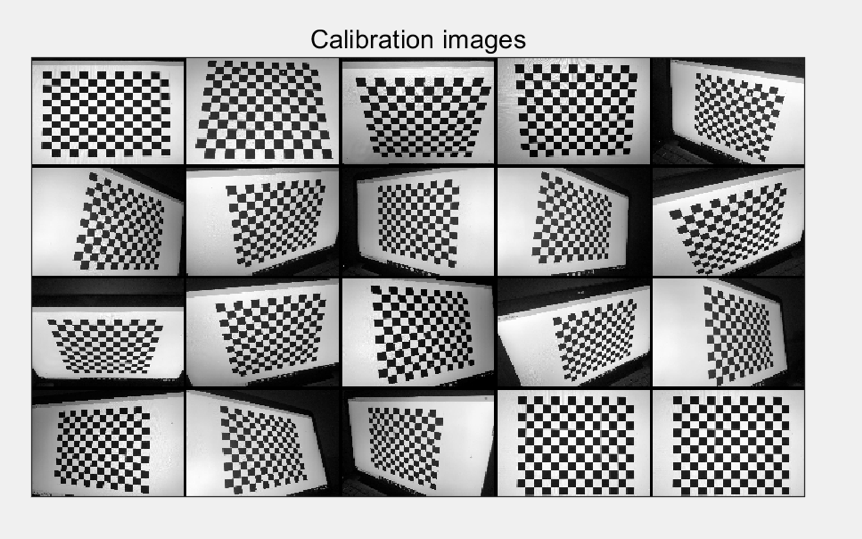
\includegraphics[width=0.7\textwidth]{figures/Picture1.png}
\subsection{去畸变}
对于想要的无畸变的目标图像,从已畸变的图像找出对应的像素,将该像素颜色填入目标图像,以此构建像素映射完成去畸变图像

\subsection{SURF}
SURF(Speeded Up Robust Features, 加速稳健特征) 是一种稳健的图像识别和描述算法。它是SIFT的高效变种,也是提取尺度不变特征,算法步骤与SIFT算法大致相同,但采用的方法不一样,要比SIFT算法更高效(正如其名)。SURF使用海森(Hesseian)矩阵的行列式值作特征点检测并用积分图加速运算;SURF 的描述子基于 2D 离散小波变换响应并且有效地利用了积分图

算法步骤:
\begin{enumerate}
    \item \textbf{特征点检测}:SURF使用Hessian矩阵来检测特征点,该矩阵是x,y方向的二阶导数矩阵,可测量一个函数的局部曲率,其行列式值代表像素点周围的变化量,特征点需取行列式值的极值点。用方型滤波器取代SIFT中的高斯滤波器,利用积分图(计算位于滤波器方型的四个角落值)大幅提高运算速度
    \item \textbf{特征点定位}:与SIFT类似,通过特征点邻近信息插补来定位特征点
    \item \textbf{方向定位}:通过计算特征点周围像素点x,y方向的哈尔小波变换,并将x,y方向的变换值在xy平面某一角度区间内相加组成一个向量,在所有的向量当中最长的(即x、y分量最大的)即为此特征点的方向。
    \item \textbf{特征描述子}:选定了特征点的方向后,其周围相素点需要以此方向为基准来建立描述子。此时以$5\times5$个像素点为一个子区域,取特征点周围$20\times20$个像素点的范围共16个子区域,计算子区域内的$x$、$y$方向(此时以平行特征点方向为x、垂直特征点方向为$y$)的哈尔小波转换总和$\sum dx$、$\sum dy$与其向量长度总和$\sum \vert dx\vert$、$\sum\vert dy\vert$共四个量值,共可产生一个64维的描述子。
\end{enumerate}

\subsection{RANSAC}

在经典的RANSAC流程中,目标函数$C$可以被看作:在第k次迭代过程中,在当前变换参数$\theta_k$作用下,数据集中满足变换参数的点的个数,也就是在当前变换条件下类内点的个数,而RANSAC就是最大化$C$的的过程。而判断当前某个点是否为类内需要一个阈值$t$。

在迭代的过程中,当前变换参数$\theta$的计算需要$U$中的一个子集$ I $来计算,RANSAC是一个随机从$U$中采样一个子集,然后对参数“估计-确认”的循环。每一个子集应是一个大小为$m$ 的最小采样。所谓最小采样,就是$m$ 的大小刚好满足计算$\theta$的个数即可。
在置信度为$\eta_0$的条件下,在循环过程中,至少有一次采样,使得采样出的$m $个点均为类内点,这样才能保证在循环的过程中,至少有一次采样能取得目标函数的最大值。因此,采样次数$k$应该满足以下条件:

$$
    k>\frac{\log(1-\eta_0)}{\log(1-\epsilon^m)}
$$

这里除了置信度$\eta_0$外,$m $为子集大小,$\epsilon$为类内点在$u$中的比例,其中置信度一般设置为[0.95, 0.99]的范围内。然而在一般情况下,$\epsilon$显然是未知的,因此 $\epsilon$可以取最坏条件下类内点的比例,或者在初始状态下设置为最坏条件下的比例,然后随着迭代次数,不断更新为当前最大的类内点比例。

\subsection{三角化进行点云重构原理}
三角化的过程即为在已知两个成像平面中对应的点位置$(x,x^\prime)$的情况下,如果知道两个成像视角的相机矩阵$(y,y^\prime)$,就可以重构出该对应点在三维空间中的位置

\subsection{Bundle Adjustment}
BA是一个图优化模型, 优化的是这个图模型的节点由相机$P_i$和三维空间点构成$X_j$构成,如果点$X_j$投影到相机$P_i$的图像上则将这两个节点连接起来。

\begin{center}
    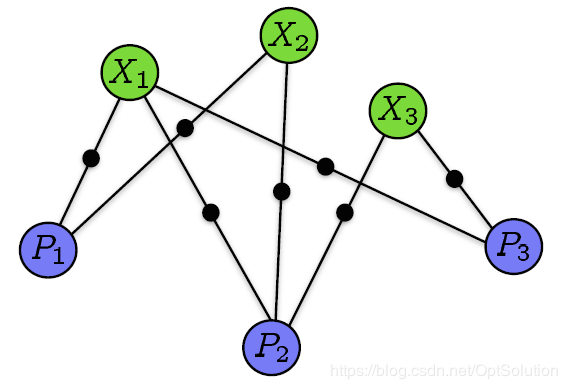
\includegraphics[width=0.6\textwidth]{figures/BA.png}
\end{center}


令点$X_j$在相机$P_i$拍摄到的图像归一化坐标系傻姑娘的坐标为$k(u_{ij}^T,1)^T = K_i^{-1}x_{ij}$, 其重投影后的图像归一化坐标系下坐标为$k^\prime(u_{ij}^T,1)^T=K_i^{-1}P_iX_j$,其中$K_i^{-1}$是为了在计算时能够不受相机内参数的影响$k$和$k^\prime$是将齐次坐标转换为非齐次坐标的常数项,可以得到该重投影误差为
$$
e_{ij} = u_{ij}-v_{ij}
$$
BA就是要将所有的重投影误差的和最小化:
$$
min_{R_i,t_i,X_j}\sum_{i,j}\sigma_{ij}\vert\vert u_{ij}-v_{ij}\vert\vert_2
$$

\chapter{Code}
\label{chap: Code}

\section{相机内参标定实现}
利用MATLAB的“TOOLBOX\_calib”工具包在输入了标定图片之后会自动标定。标定得到的相机参数如图所示:

\begin{center}
    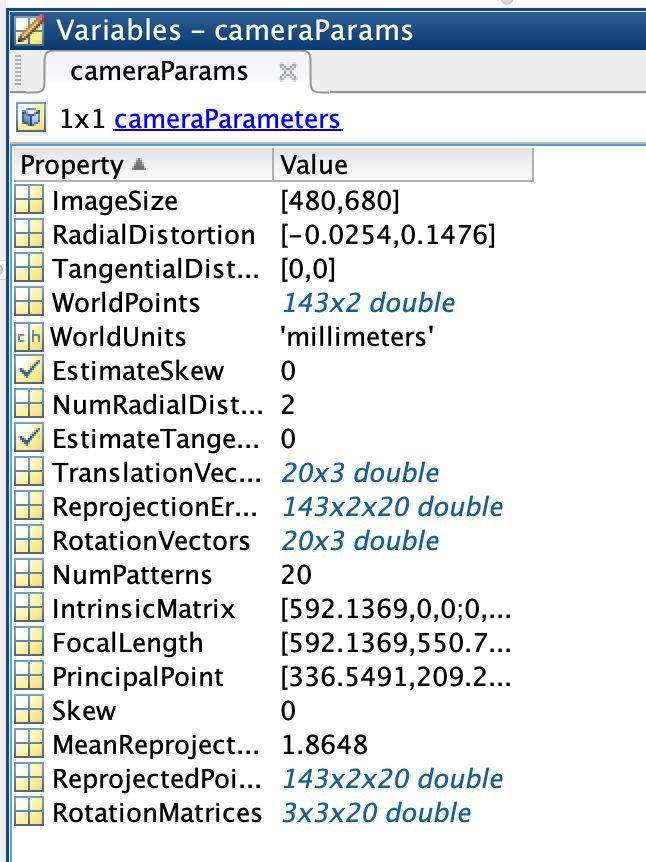
\includegraphics[width=0.4\textwidth]{figures/camera.png}
\end{center}

\section{去畸变}
MATLAB自带去除畸变的函数unditorImage,输入相机内参以及由该相机拍摄的图片即可获得去畸变处理后的图像

\begin{lstlisting}
I1 = undistortImage(I1,mycamera);
I2 = undistortImage(I2,mycamera);
I3 = undistortImage(I3,mycamera);
\end{lstlisting}


\section{特征点匹配}
在实际检测特征点的时候使用了SURF算子,对两张图片首先分别利用detectSURFFeatures函数检测图像的SURF特征点,该函数输入为需要提取特征的图像,返回提取得到的SURF特征点。然后利用extractFeatures函数对上一步提取得到的特征点计算描述向量用于之后的匹配。

extractFeatures函数的输入为图片以及对应的特征点,返回值为SURF描述子(特征描述向量)以及对应该描述子的点的位置。

\begin{lstlisting}
SURF_Pt_1 = detectSURFFeatures(rgb2gray(I1));
SURF_Pt_2 = detectSURFFeatures(rgb2gray(I2));
[features_1,validPoints_1] = 
    extractFeatures(rgb2gray(I1),SURF_Pt_1);
[features_2,validPoints_2] =   
    extractFeatures(rgb2gray(I2),SURF_Pt_2);
\end{lstlisting}

利用描述子做匹配的过程主要运用了matchFeatures函数,该函数输入为两个图像的特征描述子,返回的是匹配之后的匹配点的索引,index,其中index为n*2的矩阵,第一列对应第一张图像的匹配点的索引,第二列对应第二张图像的匹配点的索引。有了该索引,结合extractFeatures函数输出的描述向量对应点的位置,即可得到两张图片的匹配点。在匹配的过程中,为了降低outlier的比例,利用最佳匹配和第二好匹配的特征描述子距离比值进行筛选,对应于matchFeatures函数的'Maxratio'参数,在这里按照老师的建议设置为0.7。在得到了匹配点的位置之后就可以进行显示,显示函数为showMatchedFeatures。

\section{使用RANSAC进行基础矩阵的估算}
利用RANSAC进行基础矩阵及本征矩阵的估算的实现,可以调用Computer Vision System Toolbox 工具箱中的estimateFundamentalMatrix和estimateEssentialMatrix函数。
我利用第4步求出的匹配点集,调用estimateFundamentalMatrix函数,该函数的输入为两组相互匹配的点集,以及一些(name,value)对,在这里设置’Method’为‘RANSAC’,即使用RANSAC方法对该匹配进行基础矩阵求解。该函数在返回基础矩阵F的同时还返回了对应于该基础矩阵的内点。在这个迭代过程之后,将返回的内点送入estimateEssentialMatrix函数再计算一遍本征矩阵,由于输入已经是内点,且考虑时间成本,该计算过程不需要RANSAC迭代,可直接得到对于本征矩阵E的较精确的估计。

\begin{lstlisting}
[F, inliers] = estimateFundamentalMatrix(
    matchedPoints1_12,matchedPoints2_12,'Method','RANSAC');
inlierPoints1_12 = 
    matchedPoints1_12(inliers,:);
inlierPoints2_12 = 
    matchedPoints2_12(inliers,:);
figure;
showMatchedFeatures(I1, I2, inlierPoints1_12,
    inlierPoints2_12,'montage','PlotOptions',{'ro','go','y--'});
title('Point matches after outliers were removed');
%重新把inliner拿去重新算一遍Fundamental Matrix
[F,inliers] = estimateFundamentalMatrix(
    inlierPoints1_12, inlierPoints2_12, 'Method', 'RANSAC');
\end{lstlisting}

\section{从基础矩阵中分解旋转矩阵与平移矩阵}
显然在通过两个图像点的匹配求得对应的本征矩阵之后,可直接由本征矩阵结合相机参数估算两个视角的相对旋转矩阵与平移矩阵。该过程可利用MATLAB中的relativeCameraPose函数和cameraPoseToExtrinsics函数。其中relativeCameraPose函数输入为本征矩阵、相机内参以及对应的匹配内点。该函数的作用即将联系两张图像的本征矩阵转化成对应的相机相对位置。返回的参数即相对方向和相对距离。将这两个返回参数送入cameraPoseToExtrinsics函数就可以将该相对方向和距离转化为相对旋转矩阵和平移矩阵。对于第一张图像的相机位姿而言,它在这个过程中是起到参照物的作用,因此它的相对方向和距离矩阵分别为单位阵和零矩阵。将单位阵和零矩阵输入cameraPoseToExtrinsics函数便可得到在第一个相机位姿的参照下,其本身的旋转矩阵和平移矩阵。

\begin{lstlisting}[language=matlab]
Ori1 = [1,0,0; 0,1,0; 0,0,1];
Loc1 = [0,0,0];
[M_rot1, M_trans1] = cameraPoseToExtrinsics(Ori1, Loc1);

[reOri_12, reLoc_12] = relativeCameraPose(
    F, mycamera, inlierPoints1_12, inlierPoints2_12);
[M_rot2, M_trans2] = 
    cameraPoseToExtrinsics(reOri_12, reLoc_12);
\end{lstlisting}

\section{三角化三维点云重构}
当我们知道两张图像的对应匹配点,同时还得到了两个成像相机的相机矩阵,就可以用三角法重构出这些点在三维坐标下的位置。在MATLAB实现的过程中,调用了cameraMatrix函数,输入相机参数以及对应的相机的旋转矩阵和平移矩阵,返回该相机矩阵。对两个相机位姿拍下的图分别调用该函数,即可得到两个相机矩阵,将相机矩阵与两张图中的匹配点输入triangulate函数进行三角化,即可得到在三维坐标系下各点的位置

\begin{lstlisting}
Cam1 = cameraMatrix(cameraParams, eye(3), [0 0 0]);
Cam2 = cameraMatrix(mycamera,M_rot2,M_trans2);
worldPoint = triangulate(
    matchedPoints1_12,matchedPoints2_12,Cam1,Cam2);
\end{lstlisting}

\section{得到第三张图的3D-2D对应关系}
我已经得到了在第一个相机参照下的三维点云,我们再对第一张图片与第三张进行SURF特征匹配,并根据匹配点在三维坐标系下的坐标得到对应第三个相机的部分点在三维坐标系下的坐标,由于我们的三维坐标系是以第一个相机为中心建立的,因此由这些点在三维坐标系下的位置我们又可以估算第三个相机相对第一个相机的位姿。

\begin{lstlisting}
SURF_Pt_3 = detectSURFFeatures(rgb2gray(I3));
[features_3,validPoints_3] = 
    extractFeatures(rgb2gray(I3),SURF_Pt_3);
indexPairs2 = matchFeatures(features_1, 
    features_3, 'MaxRatio', 0.7, 'Unique', true);
matchedPoints1_13 = validPoints_1(indexPairs2(:,1));
matchedPoints3_13 = validPoints_3(indexPairs2(:,2));
[asd,index12_1,index13_1] = 
    intersect(indexPairs(:,1),indexPairs2(:,1));
worldPoint_i3 = worldPoint(index12_1,:);
pixelPoint_i3 = 
    matchedPoints3_13(index13_1,:).Location;
\end{lstlisting}


\section{使用RANSAC方法估算第三个视角位置}
我们已经知道了第三张图片的点在三维空间中的坐标,我们就可以利用MATLAB的estimateWorldCameraPose函数估算出在三维空间里的相机3的方向与距离矢量。由于我们的三维空间是以第一个相机的位姿为中心建立的,因此这个位姿就是相机3相对相机1的位姿(对应P3P算法)。在MATLAB实现过程中首先用estimateWorldCameraPose函数估算相机3在三维空间里的方向和距离,再利用cameraPoseToExtrinsics函数得到该方向和距离对应的旋转矩阵和平移矩阵。

\begin{lstlisting}
[reOri_13, reLoc_13] = estimateWorldCameraPose(
    pixelPoint_i3,worldPoint_i3,mycamera);
[M_rot3, M_trans3] = 
    cameraPoseToExtrinsics(reOri_13, reLoc_13);
Cam3 = cameraMatrix(mycamera,M_rot3,M_trans3);
\end{lstlisting}
    

\chapter{Result}
\label{chap:Result}

\section{Result}
首先是观察SURF初步匹配的情况。

\begin{center}
    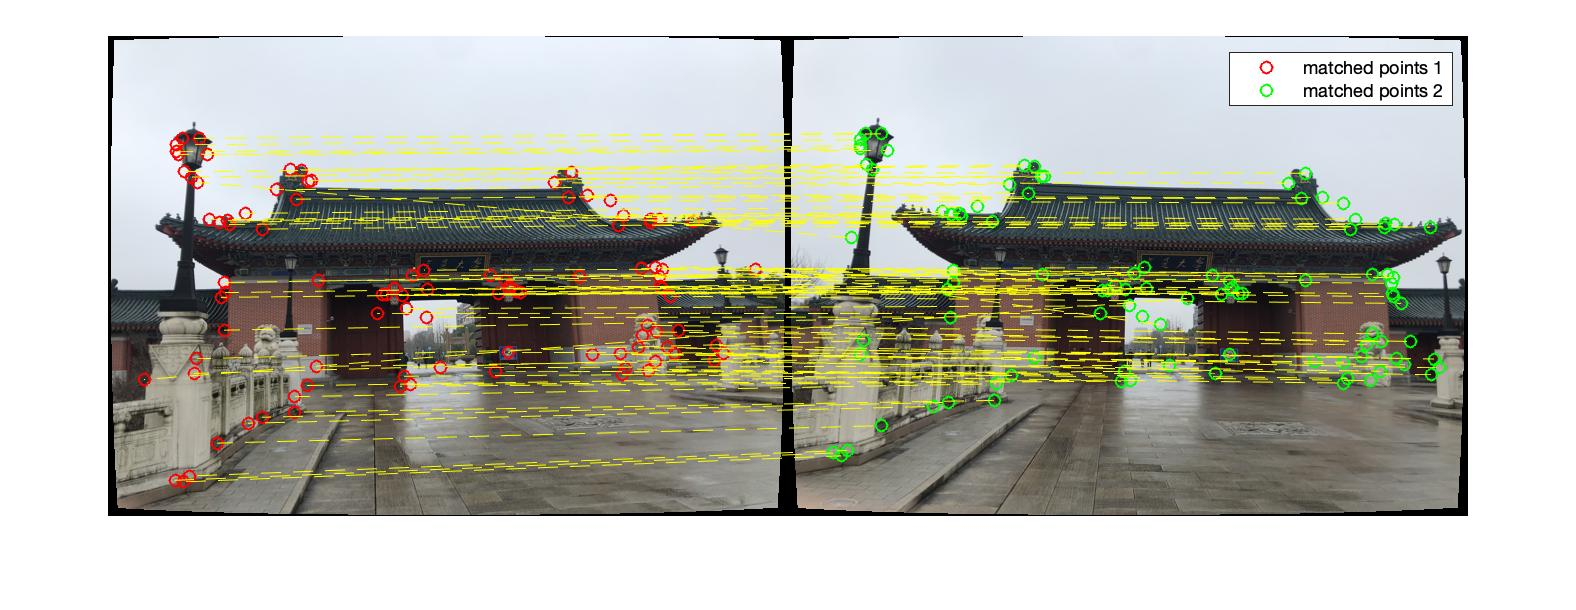
\includegraphics[width=0.9\textwidth]{figures/1.jpg}
\end{center}

我们可以发现图片的边界有一点变化,这是由于做完畸变矫正的原因。其次我们可以看到大部分的对应点都是相互对应的。表现比较好

接下来我们再看一下做完了RANSEC之后的结果。
\begin{center}
    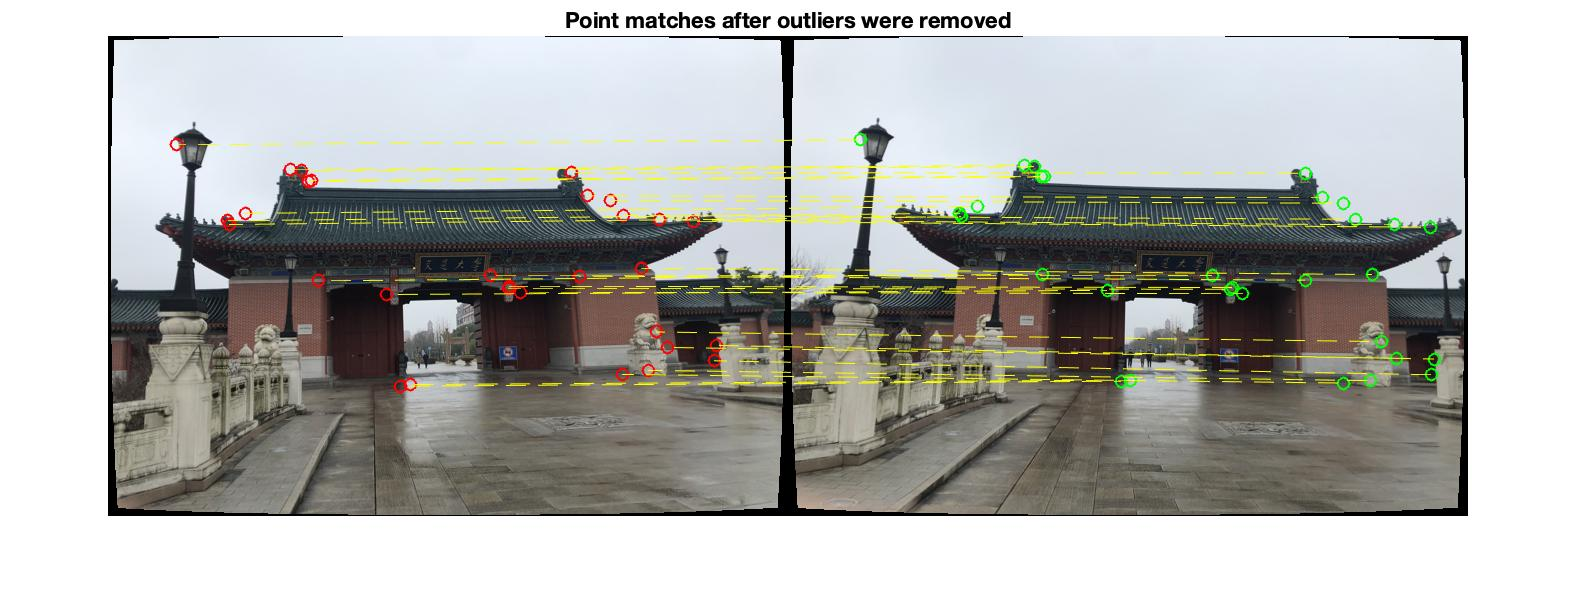
\includegraphics[width=0.9\textwidth]{figures/2.jpg}
\end{center}

发现对应点变少了,但是对应关系依旧是非常的好。
再看一下点云图
\begin{center}
    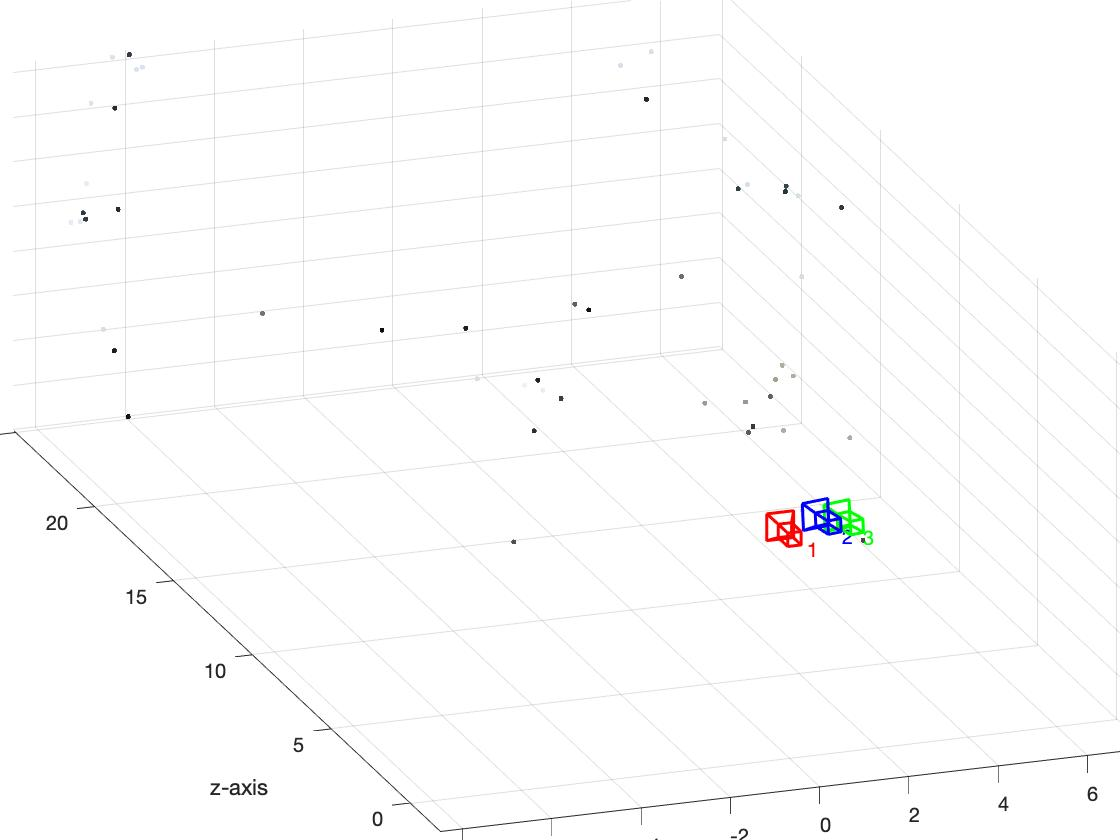
\includegraphics[width=0.9\textwidth]{figures/3.jpg}
\end{center}
可以看到,将特征点与相机位置放到三维坐标系下,可以定性地看出拍照时的实际站位关系,三个相机位置基本正确,特征点的位置也是相对正确的。

最后在看一下经过了bundle Adjustment之后的结果图
\begin{center}
    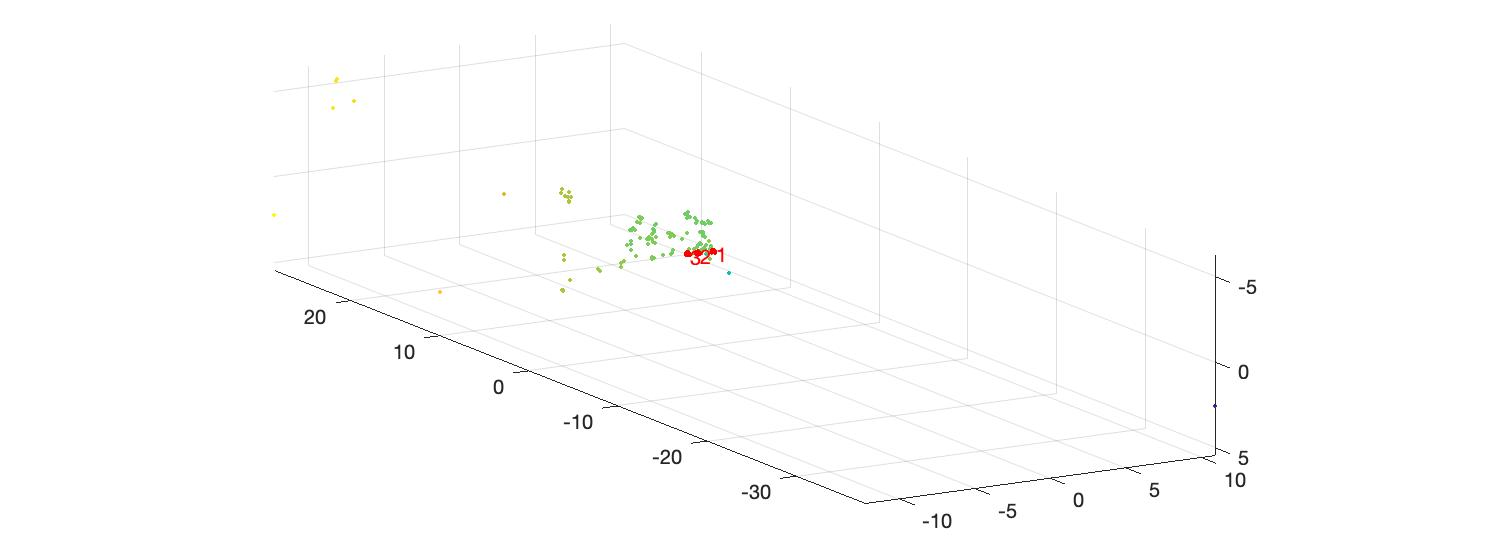
\includegraphics[width=0.9\textwidth]{figures/bundleadjustment.jpg}
\end{center}

\section{量化分析}
在此使用另外一种方法计算第三个相机视角。就是直接使用第一张图和第三张图进行匹配,求出相对位置关系。

原来的结果和使用直接匹配的方法求出来的结果分别为:
\begin{center}
    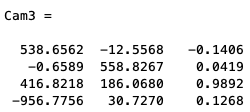
\includegraphics[width=0.4\textwidth]{figures/test1.png}
    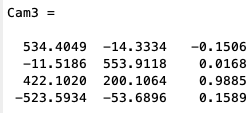
\includegraphics[width=0.4\textwidth]{figures/test2.png}
\end{center}
可以发现,基本上除了少许的一两个值变化比较大,其他的值几乎是没有什么变化,这个不同是由于在匹配的时候原来的方法使用的是已经经过匹配的特征点进行匹配的,精度会比直接匹配来的精确,这也是造成这个差别的原因。



% \include{chapters/04-chapter}

% References
\clearpage
% \addcontentsline{toc}{chapter}{Bibliography}
% \markboth{\MakeUppercase{Bibliography}}{}
% \singlespacing
% \printbibliography

% \appendix
% \chapter{Title of Appendix A}

Lorem Ipsum

\end{document}